% Compile from this directory using LuaLaTeX; assets/ is required.
\documentclass[11pt,a4paper,landscape]{ltjsarticle}
\usepackage[margin=14mm,footskip=7mm]{geometry}
\usepackage{luatexja-fontspec}
\setmainfont{arial.ttf}[Path=C:/Windows/Fonts/,BoldFont=arialbd.ttf,ItalicFont=ariali.ttf,BoldItalicFont=arialbi.ttf]
\setsansfont{arial.ttf}[Path=C:/Windows/Fonts/,BoldFont=arialbd.ttf]
\setmainjfont{YuGothM.ttc}[Path=C:/Windows/Fonts/,FontIndex=0,BoldFont=YuGothB.ttc,BoldFeatures={FontIndex=0}]
\setsansjfont{YuGothM.ttc}[Path=C:/Windows/Fonts/,FontIndex=0,BoldFont=YuGothB.ttc,BoldFeatures={FontIndex=0}]
\usepackage{graphicx,xcolor,booktabs,array,amsmath}
\usepackage{hyperref}
\hypersetup{unicode=true,hidelinks,pdftitle={CIM出力解の多様性：既存実験の再解析},pdfauthor={}}
\definecolor{ink}{HTML}{263D50}
\definecolor{accent}{HTML}{C34436}
\definecolor{light}{HTML}{F1F5F8}
\definecolor{muted}{HTML}{596874}
\setlength{\parindent}{0pt}
\setlength{\parskip}{5pt}
\setlength{\tabcolsep}{9pt}
\renewcommand{\arraystretch}{1.3}
\newcommand{\heading}[2]{\noindent{\small\color{muted} CIM研究・相談資料\hfill 2026年9月14日}\par\vspace{1mm}{\LARGE\bfseries\color{ink} #1}\par{\small\color{muted}#2}\par\vspace{2mm}}
\newcommand{\boxnote}[1]{\begingroup\setlength{\fboxsep}{8pt}\colorbox{light}{\parbox{\dimexpr\linewidth-16pt\relax}{#1}}\endgroup}
\renewcommand{\strong}[1]{{\bfseries\color{ink}#1}}
\newcommand{\smallnote}[1]{{\footnotesize\color{muted}#1\par}}
\begin{document}

\heading{CIM出力解の多様性を、なぜ調べるのか}{既存のGA収束図とCIM解集合の再解析から、研究の根拠を整理する}
\boxnote{\strong{今回確認できたこと：}カット値の分布を完全にそろえたCIM解集合でも、多様性は異なる。\\
\strong{位置づけ：}多様性をCIM出力の評価軸として調べる根拠になる。GA性能への因果効果は、次の検証対象である。}
\vspace{3mm}

\begin{minipage}[t]{0.65\linewidth}
\vspace{0pt}
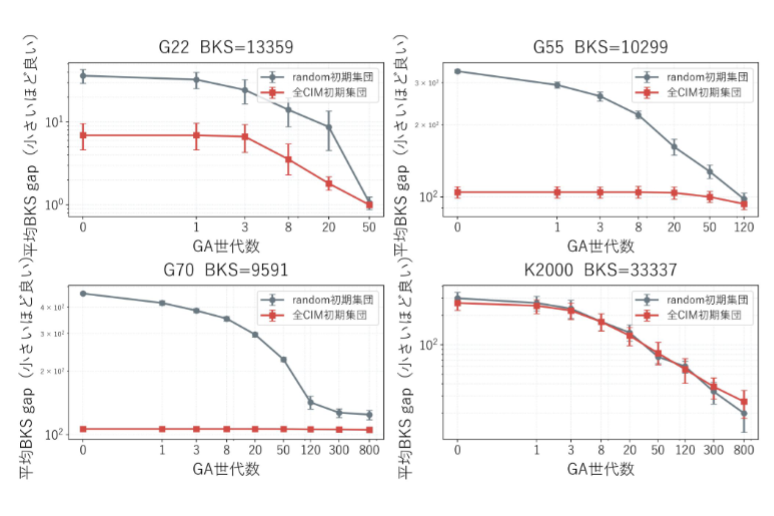
\includegraphics[width=\linewidth]{assets/original_screenshot.png}
\smallnote{図1．提供されたGA収束図をそのまま掲載。縦軸は図中表記の平均BKS gap、横軸はGA世代数。画像から数値の補間・推定はしていない。}
\end{minipage}\hfill
\begin{minipage}[t]{0.32\linewidth}
\vspace{0pt}
\strong{観測から立てる問い}

G55・G70では、全CIM初期集団は序盤から良い値を持つ一方、その後の改善は小さい。G22・K2000では、CIM初期集団にも改善が見られる。

この違いから、初期カット値に加えて\strong{解集合の構造}を調べる動機が得られる。

\strong{この図だけで分からないこと}

多様性そのものは表示されていない。したがって、停滞を多様性不足だけで説明することは、まだできない。

\smallnote{元データ未確認のため、試行数・誤差棒の定義・世代0の処理内容は不明。今回のCIM再解析とは別実験として扱う。}
\end{minipage}

\clearpage
\heading{結果1：品質と多様性を並べて評価する}{基準CIMとノイズ振幅1,000倍の比較。各条件32試行を使用}
\begin{center}
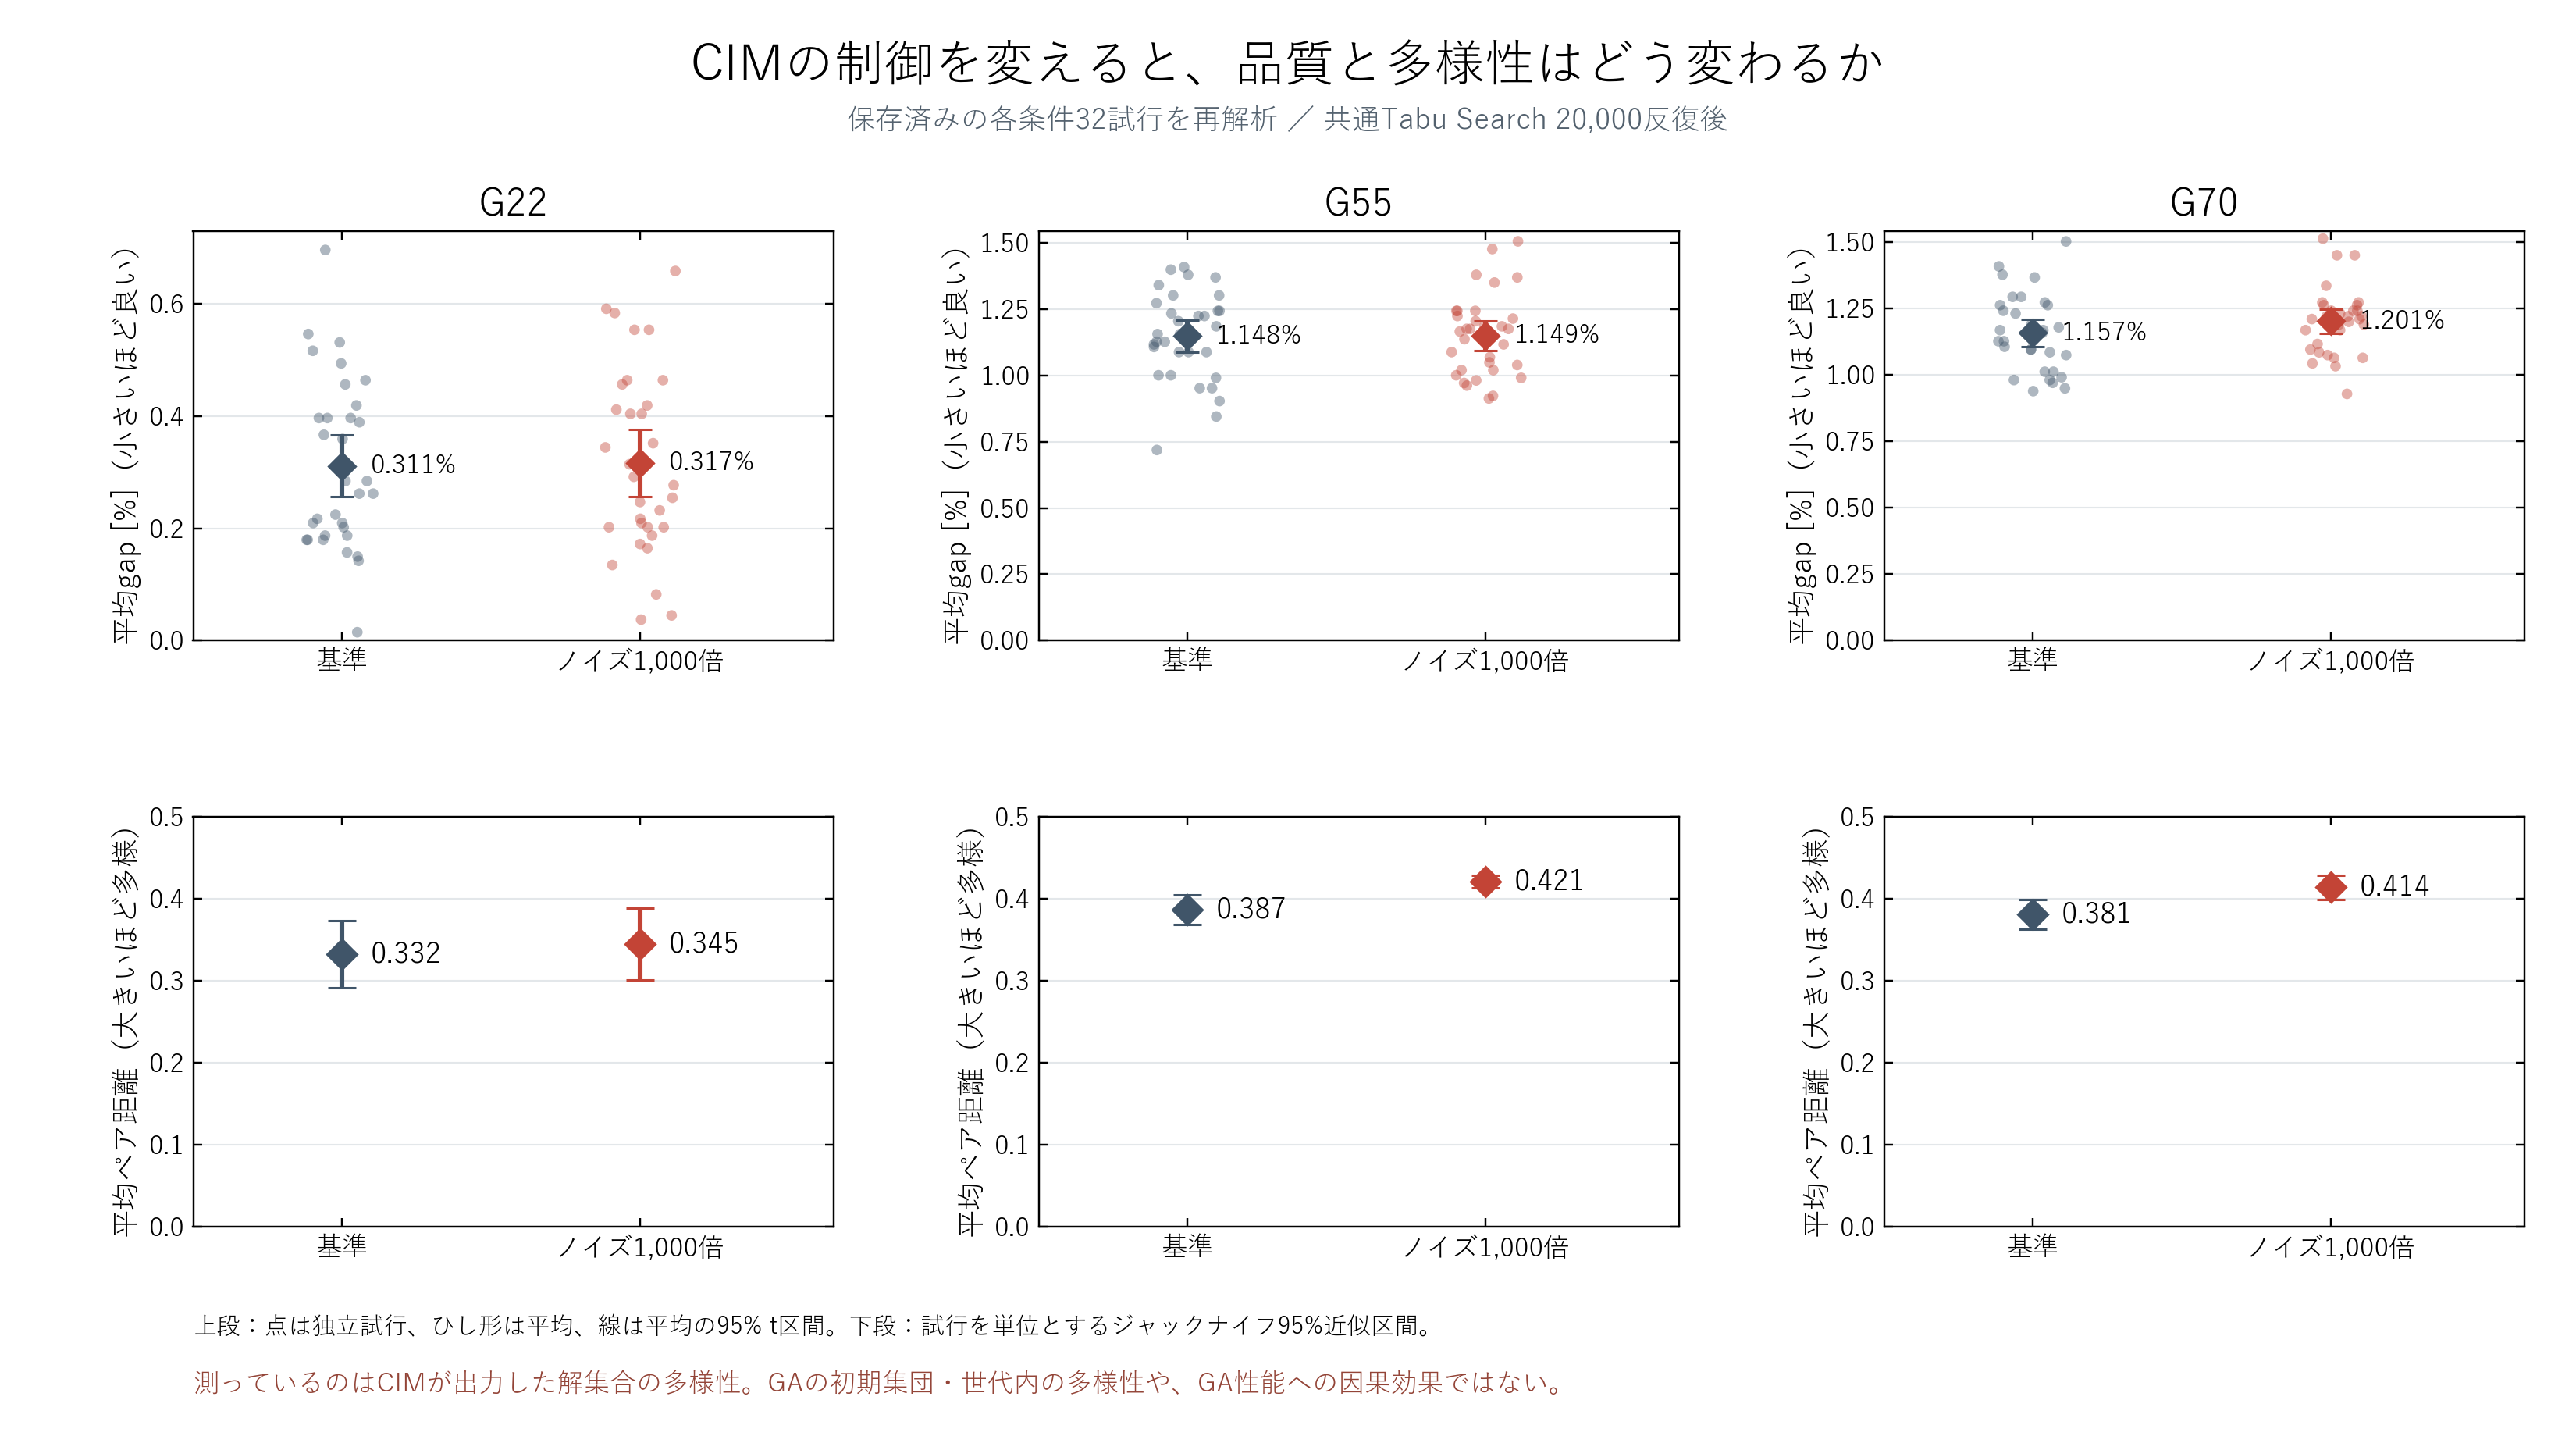
\includegraphics[width=\linewidth,height=130mm,keepaspectratio]{assets/01_quality_and_diversity.png}
\end{center}
\smallnote{図2．共通Tabu Search（20,000反復、摂動なし）後の保存解を再解析。G55では平均gapがほぼ同じでも、平均ペア距離が異なる。G70は距離増加と小幅な平均gap悪化が併存し、G22で差は小さい。集団の品質と多様性を分けて読む。}

\clearpage
\heading{結果2：カット値の分布を完全一致させる}{各カット値について、2条件から同じ数の解を抽出。平均だけでなく分布をそろえる}
\begin{center}
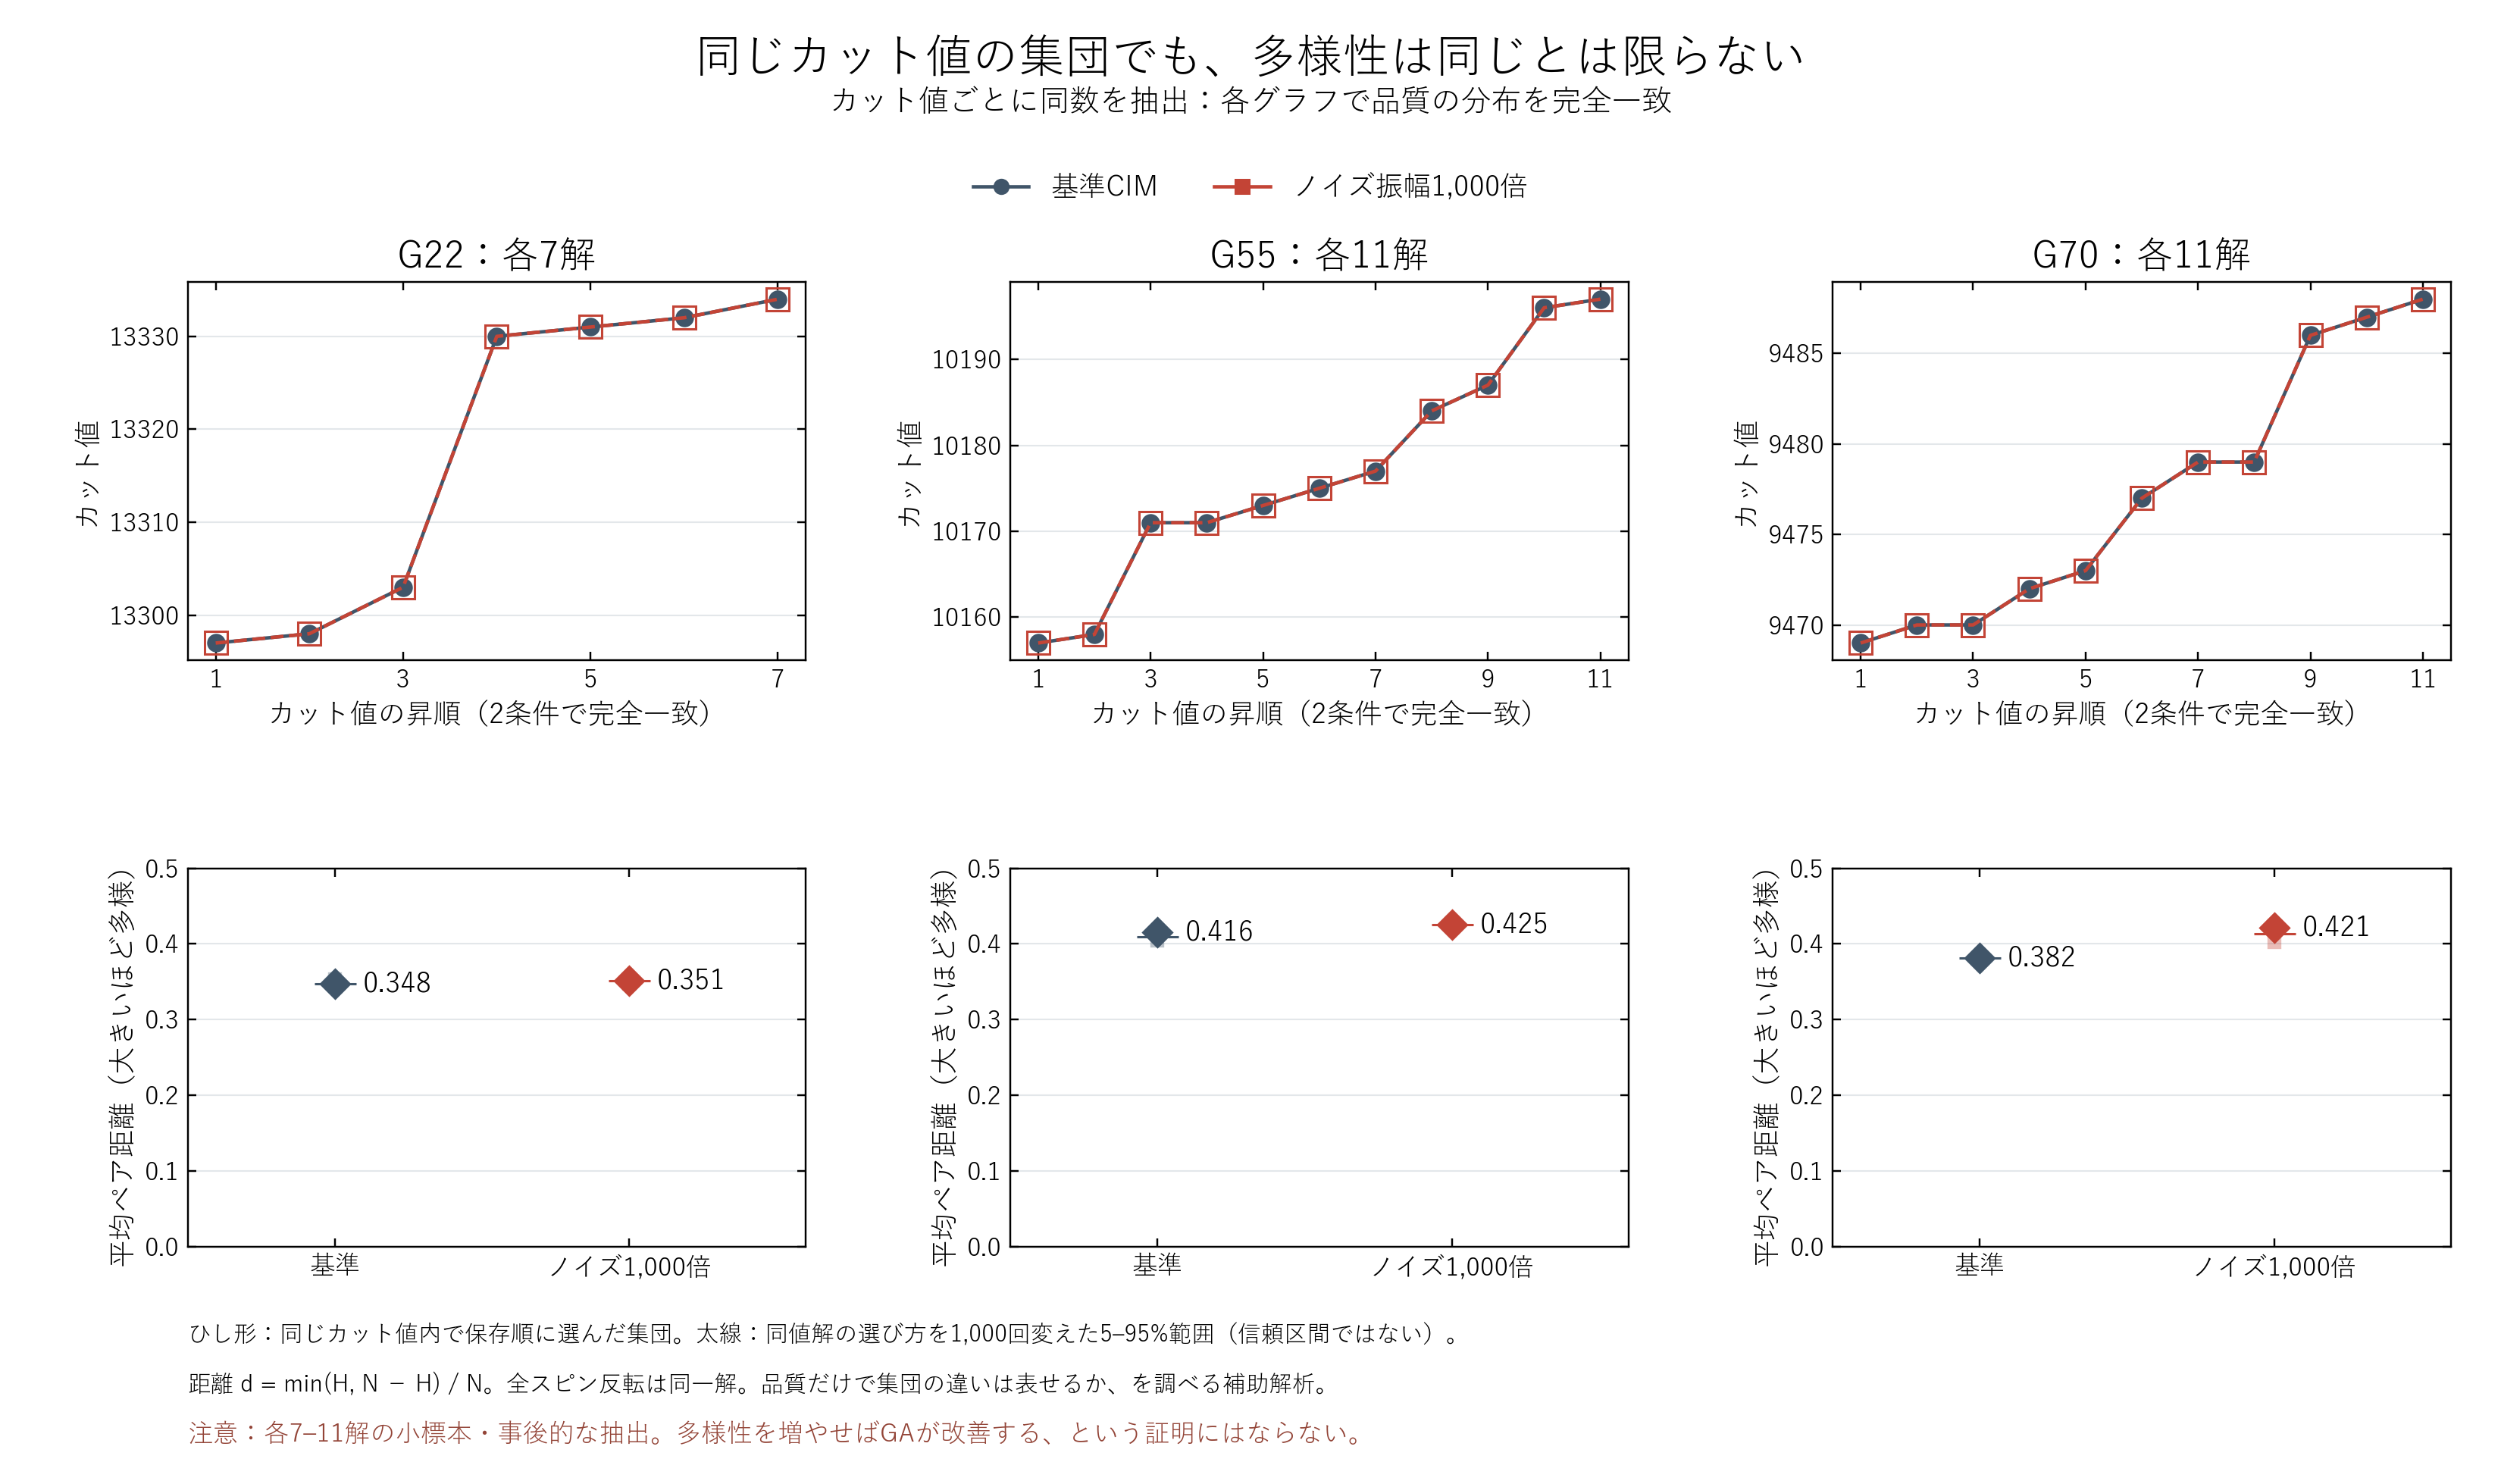
\includegraphics[width=\linewidth,height=130mm,keepaspectratio]{assets/02_exact_quality_matching.png}
\end{center}
\smallnote{図3．G70は各11解の平均カット値が共に9,477.273でも、平均距離は0.3817と0.4213。品質だけで集合の違いを表せないことを示す。抽出は保存順で決め、距離を使って選別していない。小標本の事後解析であり、GA性能への効果は未評価。}

\clearpage
\heading{結果3：品質とのトレードオフも確認する}{ノイズ条件だけに限定せず、8月23日の全15条件を比較する}
\begin{center}

\includegraphics[width=\linewidth,height=99mm,keepaspectratio]{assets/03_all_conditions.png}
\end{center}
\vspace{1mm}
\begin{minipage}[t]{0.49\linewidth}
\strong{多様性が大きいだけでは十分ではない}

ポンプ速度を変えた条件には、多様性の増加に品質低下が伴うものがある。目標は、\strong{高品質な解の間に有用な違いを作ること}である。

全15条件には、基準、初期振幅3条件、ポンプ速度4条件、ノイズ3条件、更新方式4条件が含まれる。
\end{minipage}\hfill
\begin{minipage}[t]{0.47\linewidth}
\strong{今回の多様性の定義}
\[
d(s,u)=\frac{\min\{H(s,u),\,N-H(s,u)\}}{N},
\qquad
D=\frac{2}{M(M-1)}\sum_{i<j}d(s_i,s_j).
\]
\smallnote{$H$：ハミング距離、$N$：頂点数、$M$：解数。Max-Cutでは全スピン反転が同じ分割を表すため、その対称性を除いて計算する。$D$は0から0.5の範囲。}
\end{minipage}

\clearpage
\heading{先生への説明と、次に確かめること}{研究対象はCIMの解形成と制御。GAは生成した解集合の有用性を評価するために使う}

\begin{minipage}[t]{0.53\linewidth}
\strong{説明例}

\boxnote{全CIM初期集団は初期の品質が良い一方、G55・G70ではその後の改善が小さくなっています。そこで初期カット値以外の性質を調べました。保存済みのCIM解では、カット値の分布をそろえても多様性が異なります。これを根拠に、多様性をCIM出力の評価軸として加え、その形成機構と制御を研究したいと考えています。}

\vspace{3mm}
\strong{同品質部分集合の数値}

{\small
\begin{tabular}{lrrrr}
\toprule
グラフ & 各解数 & 共通の平均cut & 基準の$D$ & ノイズの$D$\\
\midrule
G22 & 7 & 13,317.857 & 0.3476 & 0.3512\\
G55 & 11 & 10,176.909 & 0.4158 & 0.4254\\
G70 & 11 & 9,477.273 & 0.3817 & 0.4213\\
\bottomrule
\end{tabular}}

\smallnote{全32試行からの抽出。ノイズは振幅1,000倍条件。同じカット値内の解を選び直した感度は図3に表示し、信頼区間とは区別した。}
\end{minipage}\hfill
\begin{minipage}[t]{0.43\linewidth}
\strong{GAへの効果を確かめる比較}

\begin{enumerate}
\setlength{\itemsep}{3pt}
\item 同じ品質分布・同じ集団サイズで、距離の低い集団と高い集団を複数作る。
\item 同じGA、同じ計算予算、対応する乱数で比較する。
\item 初期局所探索の前後・各世代で品質と多様性を記録する。交叉直後と局所探索後の改善を分ける。
\end{enumerate}

\smallnote{CIM生成条件を変えると、多様性以外の構造も変わる。複数の生成条件や集団構成で結果が続くか調べる。今回、GAの追加実行は行っていない。}

\strong{統計と検証の扱い}

\smallnote{図2上段は平均の95\% $t$区間、下段は試行単位の削除1ジャックナイフによる95\%近似区間。496個のペアを独立標本として扱っていない。カット値は元のグラフから独立に再計算し、距離は保存JSONと照合済み。}
\end{minipage}

\vfill
\hrule
\vspace{2mm}
\smallnote{資料A：ユーザー提供スクリーンショット（2026-09-13 23:56:15）。対応する全CIM実験の元データは未確認。2026-09-14のpull時点でmasterは\texttt{bb5f62d}（2026-08-24）。}
\smallnote{資料B：\nolinkurl{results/2026-08-23/cim_diversity_ablation/v3_G22_G55_G70_nt32_ex1234_main/} 内の\texttt{signs\_ref20k.npz}・\texttt{results\_ref20k.json}。}
\smallnote{再解析：\nolinkurl{scripts/plotting/plot_cim_diversity_evidence.py}。抽出メンバー、集計、元データのSHA-256は\texttt{cim\_diversity\_evidence/v2\_G22\_G55\_G70\_matched\_r1000\_discussion}に保存。}

\end{document}
